\documentclass{article}
\usepackage[utf8]{vietnam}

\title{K-nearest neighbors}
\author{Lê Doãn Hoàng Long - 1411158 \\ Lưu Minh Chí - 18110065}
\date{Tháng 12 năm 2020}

\usepackage{natbib}
\usepackage{graphicx}

\usepackage{listings}
\usepackage{color}

\definecolor{dkgreen}{rgb}{0,0.6,0}
\definecolor{gray}{rgb}{0.5,0.5,0.5}
\definecolor{mauve}{rgb}{0.58,0,0.82}

\lstset{frame=tb,
  language=Python,
  aboveskip=3mm,
  belowskip=3mm,
  showstringspaces=false,
  columns=flexible,
  basicstyle={\small\ttfamily},
  numbers=none,
  numberstyle=\tiny\color{gray},
  keywordstyle=\color{blue},
  commentstyle=\color{dkgreen},
  stringstyle=\color{mauve},
  breaklines=true,
  breakatwhitespace=true,
  tabsize=3
}

\begin{document}

\maketitle

%trang 1
\section{Giới thiệu}
K-nearest neighbor là một trong những thuật toán đơn giản nhất trong Machine Learning. Khi training, thuật toán này không học một điều gì từ dữ liệu training, mọi tính toán được thực hiện khi nó cần dự đoán kết quả của dữ liệu mới.K-nearest neighbor có thể áp dụng được vào cả hai loại của bài toán Supervised learning là Classification và Regression.

\begin{tabular}{ |c|c|c| }
\hline
Ngôn ngữ người & Ngôn ngữ Máy Học & Machine Learning \\ \hline
Câu hỏi & Điểm dữ liệu & Data point \\ \hline
Đáp án & Đầu ra, nhãn & Output, Label \\ \hline
Ôn thi & Huấn luyện & Training \\ \hline
Tập tài liệu mang vào phòng thi & Tập dữ liệu tập huấn & Training set \\ \hline
Đề thi & Tập dữ liểu kiểm thử & Test set \\ \hline
Câu hỏi trong dề thi & Dữ liệu kiểm thử & Test data point \\ \hline
Câu hỏi có đáp án sai & Nhiễu & Noise, Outlier \\ \hline
Câu hỏi gần giống & Điểm dữ liệu gần nhất & Nearest Neighbor \\
\hline
\end{tabular}
\\

Trong bài toán Classification, label của một điểm dữ liệu mới được suy ra trực tiếp từ K điểm dữ liệu gần nhất trong training set. Label của một test data có thể được quyết định bằng major voting (bầu chọn theo số phiếu) giữa các điểm gần nhất, hoặc nó có thể được suy ra bằng cách đánh trọng số khác nhau cho mỗi trong các điểm gần nhất đó rồi suy ra label.
\\

Trong bài toán Regresssion, đầu ra của một điểm dữ liệu sẽ bằng chính đầu ra của điểm dữ liệu đã biết gần nhất (trong trường hợp K=1), hoặc là trung bình có trọng số của đầu ra của những điểm gần nhất, hoặc bằng một mối quan hệ dựa trên khoảng cách tới các điểm gần nhất đó.
\\

Một cách ngắn gọn, KNN là thuật toán đi tìm đầu ra của một điểm dữ liệu mới bằng cách chỉ dựa trên thông tin của K điểm dữ liệu trong training set gần nó nhất (K-lân cận), không quan tâm đến việc có một vài điểm dữ liệu trong những điểm gần nhất này là nhiễu. Hình dưới đây là một ví dụ về KNN trong classification với K = 1.

%trang 2
\begin{center}
\begin{figure}[htp]
\begin{center}
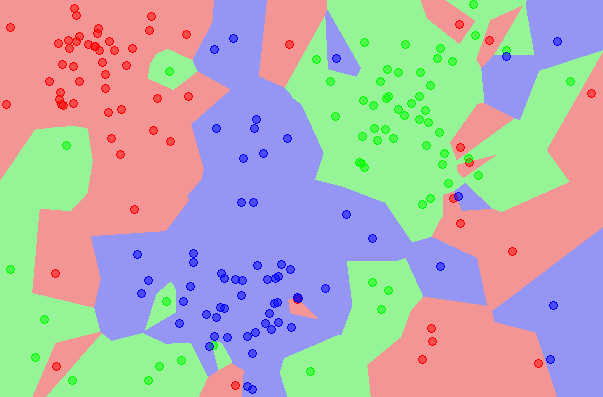
\includegraphics[scale=.7]{Map1NN}
\end{center}
\caption{Bản đồ của 1NN (Nguồn: Wikipedia)}
\label{refhinh1}
\end{figure}
\end{center}

Ví dụ trên đây là bài toán Classification với 3 classes: Đỏ, Lam, Lục. Mỗi điểm dữ liệu mới (test data point) sẽ được gán label theo màu của điểm mà nó thuộc về. Trong hình này, có một vài vùng nhỏ xem lẫn vào các vùng lớn hơn khác màu. Ví dụ có một điểm màu Lục ở gần góc 11 giờ nằm giữa hai vùng lớn với nhiều dữ liệu màu Đỏ và Lam. Điểm này rất có thể là nhiễu. Dẫn đến nếu dữ liệu test rơi vào vùng này sẽ có nhiều khả năng cho kết quả không chính xác.

\section{Ví dụ trên Python}
Iris flower dataset là một bộ dữ liệu nhỏ. Bộ dữ liệu này bao gồm thông tin của ba loại hoa Iris (một loài hoa lan) khác nhau: Iris setosa, Iris virginica và Iris versicolor. Mỗi loại có 50 bông hoa được đo với dữ liệu là 4 thông tin: chiều dài, chiều rộng đài hoa (sepal), và chiều dài, chiều rộng cánh hoa (petal).

Trong phần này, chúng ta sẽ tách 150 dữ liệu trong Iris flower dataset ra thành 2 phần, gọi là training set và test set. Thuật toán KNN sẽ dựa vào trông tin ở training set để dự đoán xem mỗi dữ liệu trong test set tương ứng với loại hoa nào. Dữ liệu được dự đoán này sẽ được đối chiếu với loại hoa thật của mỗi dữ liệu trong test set để đánh giá hiệu quả của KNN.

Trước tiên, chúng ta cần khai báo vài thư viện.

\begin{lstlisting}
import numpy as np
import matplotlib.pyplot as plt
from sklearn import neighbors, datasets
\end{lstlisting}

%trang 3
Tiếp theo, chúng ta load dữ liệu và hiện thị vài dữ liệu mẫu. Các class được gán nhãn là 0, 1, và 2.

\begin{lstlisting}
iris = datasets.load_iris()
iris_X = iris.data
iris_y = iris.target
print('Number of classes:', len(np.unique(iris_y)))
print('Number of data points:', len(iris_y))

X0 = iris_X[iris_y == 0,:]
print('\nSamples from class 0:\n', X0[:5,:])

X1 = iris_X[iris_y == 1,:]
print('\nSamples from class 1:\n', X1[:5,:])

X2 = iris_X[iris_y == 2,:]
print('\nSamples from class 2:\n', X2[:5,:])
\end{lstlisting}

Output:

\begin{lstlisting}
Number of classes: 3
Number of data points: 150

Samples from class 0:
[[ 5.1  3.5  1.4  0.2]
 [ 4.9  3.   1.4  0.2]
 [ 4.7  3.2  1.3  0.2]
 [ 4.6  3.1  1.5  0.2]
 [ 5.   3.6  1.4  0.2]]

Samples from class 1:
[[ 7.   3.2  4.7  1.4]
 [ 6.4  3.2  4.5  1.5]
 [ 6.9  3.1  4.9  1.5]
 [ 5.5  2.3  4.   1.3]
 [ 6.5  2.8  4.6  1.5]]

Samples from class 2:
[[ 6.3  3.3  6.   2.5]
 [ 5.8  2.7  5.1  1.9]
 [ 7.1  3.   5.9  2.1]
 [ 6.3  2.9  5.6  1.8]
 [ 6.5  3.   5.8  2.2]]
\end{lstlisting}

Nếu nhìn vào vài dữ liệu mẫu, chúng ta thấy rằng hai cột cuối mang khá nhiều thông tin giúp chúng ta có thể phân biệt được chúng. Chúng ta dự đoán rằng kết quả classification cho cơ sở dữ liệu này sẽ tương đối cao.
\\

%trang 4
Tách training và test sets.

Giả sử chúng ta muốn dùng 50 điểm dữ liệu cho test set, 100 điểm còn lại cho training set. Scikit-learn có một hàm số cho phép chúng ta ngẫu nhiên lựa chọn các điểm này, như sau:

\begin{lstlisting}
from sklearn.model_selection import train_test_split
X_train, X_test, y_train, y_test = train_test_split(iris_X, iris_y, test_size=50)

print('Training size:', len(y_train))
print('Test size    :', len(y_test))
\end{lstlisting}

Output:

\begin{lstlisting}
Training size: 100
Test size    : 50
\end{lstlisting}

Xét trường hợp đơn giản K = 1, tức là với mỗi điểm test data, ta chỉ xét 1 điểm training data gần nhất và lấy label của điểm đó để dự đoán cho điểm test này.

\begin{lstlisting}
clf = neighbors.KNeighborsClassifier(n_neighbors = 1, p = 2)
clf.fit(X_train, y_train)
y_pred = clf.predict(X_test)

print('Print results for 20 test data points:')
print('Predicted labels:', y_pred[20:40])
print('Ground truth    :', y_test[20:40])
\end{lstlisting}

Output:

\begin{lstlisting}
Print results for first 20 test data points:
Predicted labels:  [2 1 2 2 1 2 2 0 2 0 2 0 1 0 0 2 2 0 2 0]
Ground truth    :  [2 1 2 2 1 2 2 0 2 0 1 0 1 0 0 2 1 0 2 0]
\end{lstlisting}

Kết quả cho thấy label dự đoán gần giống với label thật của test data, chỉ có 2 điểm trong số 20 điểm được hiển thị có kết quả sai lệch.
\\

\textbf{Phương pháp đánh giá (evaluation method):}

Để đánh giá độ chính xác của thuật toán KNN classifier này, chúng ta xem xem có bao nhiêu điểm trong test data được dự đoán đúng. Lấy số lượng này chia cho tổng số lượng trong tập test data sẽ ra độ chính xác. Scikit$-$learn cung cấp hàm số accuracy$\_$score để thực hiện công việc này.

\begin{lstlisting}
from sklearn.metrics import accuracy_score
print('Accuracy of 1NN:', accuracy_score(y_test, y_pred))
\end{lstlisting}

Output:

%trang 5
\begin{lstlisting}
Accuracy of 1NN: 94.00 %
\end{lstlisting}

Nhận thấy rằng chỉ xét 1 điểm gần nhất có thể dẫn đến kết quả sai nếu điểm đó là nhiễu. Một cách có thể làm tăng độ chính xác là tăng số lượng điểm lân cận lên, ví dụ 10 điểm, và xem xem trong 10 điểm gần nhất, class nào chiếm đa số thì dự đoán kết quả là class đó. Kỹ thuật dựa vào đa số này được gọi là major voting.

\begin{lstlisting}
clf = neighbors.KNeighborsClassifier(n_neighbors = 10, p = 2)
clf.fit(X_train, y_train)
y_pred = clf.predict(X_test)

print('Accuracy of 10NN with major voting:', accuracy_score(y_test, y_pred))
\end{lstlisting}

Output:

\begin{lstlisting}
Accuracy of 10NN with major voting: 98.00 %
\end{lstlisting}

\textbf{Đánh trọng số cho các điểm lân cận}

Trong kỹ thuật major voting bên trên, mỗi trong 10 điểm gần nhất được coi là có vai trò như nhau và giá trị lá phiếu của mỗi điểm này là như nhau. Mặt khác, những điểm gần hơn nên có trọng số cao hơn (càng thân cận thì càng tin tưởng). Vậy nên ta sẽ đánh trọng số khác nhau cho mỗi trong 10 điểm gần nhất này.Cách đánh trọng số phải thoải mãn điều kiện là một điểm càng gần điểm test data thì phải được đánh trọng số càng cao (tin tưởng hơn). Cách đơn giản nhất là lấy nghịch đảo của khoảng cách này. (Trong trường hợp test data trùng với 1 điểm dữ liệu trong training data, tức khoảng cách bằng 0, ta lấy luôn label của điểm training data).

Scikit$-$learn giúp chúng ta đơn giản hóa việc này bằng cách gán gía trị \lstinline{weights = 'distance'}. (Giá trị mặc định của \lstinline{weights} là \lstinline{'uniform'}, tương ứng với việc coi tất cả các điểm lân cận có giá trị như nhau như ở trên).

\begin{lstlisting}
clf = neighbors.KNeighborsClassifier(n_neighbors = 10, p = 2, weights = 'distance')
clf.fit(X_train, y_train)
y_pred = clf.predict(X_test)

print('Accuracy of 10NN (1/distance weights):', accuracy_score(y_test, y_pred))
\end{lstlisting}

Output:

\begin{lstlisting}
Accuracy of 10NN (1/distance weights): 100.00 %
\end{lstlisting}

\textbf{Chú ý:}
\\

%trang 6
Ngoài 2 phương pháp đánh trọng số \lstinline{weights = 'uniform'} và \lstinline{weights = 'distance'} ở trên, scikit$-$learn còn cung cấp cho chúng ta một cách để đánh trọng số một cách tùy chọn. Ví dụ, một cách đánh trọng số phổ biến khác trong Machine Learning là: $w_i = \exp(\frac{-\Vert x - x_i \Vert_2^2}{\sigma^2})$.

Trong đó $x$ là test data, $x_i$ là một điểm trong K$-$lân cận của $x$, $w_i$ là trọng số của điểm đó (ứng với điểm dữ liệu đang xét $x$), $\sigma$ là một số dương. Nhận thấy rằng hàm số này cũng thỏa mãn điều kiện: điểm càng gần $x$ thì trọng số càng cao (cao nhất bằng 1). Với hàm số này, chúng ta có thể lập trình như sau:

\begin{lstlisting}
def myweight(distances):
    sigma2 = .5 # we can change this number
    return np.exp(-distances**2/sigma2)

clf = neighbors.KNeighborsClassifier(n_neighbors = 10, p = 2, weights = myweight)
clf.fit(X_train, y_train)
y_pred = clf.predict(X_test)

print('Accuracy of 10NN (customized weights):', accuracy_score(y_test, y_pred))
\end{lstlisting}

Output:

\begin{lstlisting}
Accuracy of 10NN (customized weights): 98.00 %
\end{lstlisting}

Trong trường hợp này, kết quả tương đương với kỹ thuật major voting. Để đánh giá chính xác hơn kết quả của KNN với K khác nhau, cách định nghĩa khoảng cách khác nhau và cách đánh trọng số khác nhau, chúng ta cần thực hiện quá trình trên với nhiều cách chia dữ liệu training và test khác nhau rồi lấy kết quả trung bình, vì rất có thể dữ liệu phân chia trong 1 trường hợp cụ thể là rất tốt hoặc rất xấu (bias). Đây cũng là cách thường được dùng khi đánh giá hiệu năng của một thuật toán cụ thể nào đó.

\section{Kết luận}
Với bài toán Regression, chúng ta cũng hoàn toàn có thể sử dụng phương pháp tương tự: ước lượng đầu ra dựa trên đầu ra và khoảng cách của các điểm trong K-lân cận. Việc ước lượng như thế nào các bạn có thể tự định nghĩa tùy vào từng bài toán.

\textbf{Ưu điểm của KNN}
\\
$+$ Độ phức tạp tính toán của quá trình training là bằng 0.
\\
$+$ Việc dự đoán kết quả của dữ liệu mới rất đơn giản.
\\
$+$ Không cần giả sử gì về phân phối của các class.
\\
\textbf{Nhược điểm của KNN}
\\
$-$KNN rất nhạy cảm với nhiễu khi K nhỏ.
\\
$-$Như đã nói, KNN là một thuật toán mà mọi tính toán đều nằm ở khâu test. Trong đó việc tính khoảng cách tới từng điểm dữ liệu trong training set sẽ tốn rất nhiều thời gian, đặc biệt là với các cơ sở dữ liệu có số chiều lớn và có nhiều điểm dữ liệu. Với K càng lớn thì độ phức tạp cũng sẽ tăng lên. Ngoài ra, việc lưu toàn bộ dữ liệu trong bộ nhớ cũng ảnh hưởng tới hiệu năng của KNN.

\end{document}
